\label{chap:impl}

 \subsection{Hardware Details}

The hardware components present on the SparrowDongle board are split according
to functionality. The part of the board that handles the wireless communication
has similar hardware with that of a Sparrowv3.2 wireless sensor node:

\begin{itemize}

\item RF-enabled microcontroller unit: The ATMega128RFA1 is an 8-bit
microcontroller from Atmel that has an on-chip 2.4GHz wireless transceiver.

\item On-board antenna/External antenna connector and the appropriate RF
interface circuit enables wireless communication in the 2.4GHz band

\item 16MHz MCU clock is used as the main clock domain

\item 32768 Hz real-time clock is used to keep track of tight timings in the
wireless network protocol

\end{itemize}

On the USB side, an ATMega32U4 is used as an USB Controller Unit.

Since the Radio Controller Unit needs 3.3V to operate, an additional power
supply from the USB's 5V to 3.3V is needed, as well as level adjusters for the
signals connecting the two controllers on SparrowDongle.



\begin{figure}[ht] \centering
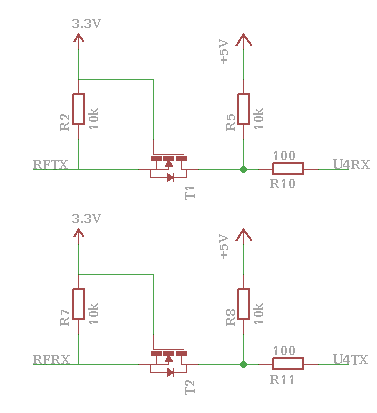
\includegraphics[width=0.35\textwidth]{img/nivel.png} \caption{Level shifters
for inter-controller communication} \end{figure}



\subsection{Software Implementation}

Software for the SparrowDongle gateway is found on the two controllers.
Firmware on the Radio Controller Unit will contain the wireless communication stack we developed for the Sparrowv3.2 wireless node.

Firmware on the USB controller unit contains the USB stack. While there are a
few libraries available for an USB stack on the ATMega32U4, our tests indicate
that the highest reliability and performance (with the smallest memory
footprint) can be obtained with "bare metal" USB code. So far the Virtual
Serial Port and Ethernet Emulation device classes have been implemented and
tested. The VirtualSerialPort works both on Windows and on Linux, while the
Ethernet Emulation device only works on Linux currently, since no open-source
drivers exist for this USB class on Windows. 


